\documentclass[12pt,a4paper]{article}

\usepackage[top=1in,bottom=1in,left=1.25in,right=1in]{geometry}
\renewcommand{\rmdefault}{ptm}
\usepackage{setspace}
\usepackage{graphicx}
\usepackage{tabularx}
\usepackage{booktabs}
\usepackage{array}
\usepackage{float}
\usepackage{caption}
\usepackage{hyperref}
\usepackage{tikz}
\usetikzlibrary{arrows.meta,positioning,shapes.geometric,fit,calc}
\usepackage{xcolor}
\usepackage{fancyhdr}
\usepackage{titlesec}

\onehalfspacing
\setlength{\parindent}{0pt}
\setlength{\parskip}{6pt}

\titleformat{\section}
  {\normalfont\fontsize{16}{19}\bfseries}{\thesection}{1em}{}
\titleformat{\subsection}
  {\normalfont\fontsize{14}{17}\bfseries}{\thesubsection}{1em}{}
\titleformat{\subsubsection}
  {\normalfont\fontsize{12}{15}\bfseries}{\thesubsubsection}{1em}{}

\captionsetup{font=bf,labelfont=bf}
\renewcommand{\contentsname}{Contents}

\pagestyle{fancy}
\fancyhf{}
\fancyfoot[C]{\thepage}
\renewcommand{\headrulewidth}{0pt}
\fancypagestyle{plain}{\fancyhf{}\fancyfoot[C]{\thepage}\renewcommand{\headrulewidth}{0pt}}

\hypersetup{
  colorlinks=true,
  linkcolor=black,
  citecolor=black,
  urlcolor=blue
}

\begin{document}

\hypersetup{pageanchor=false}
\begin{titlepage}
\begin{center}

\textbf{\fontsize{14}{17}\selectfont Lincoln University College}\\[4pt]
\textbf{\fontsize{12}{15}\selectfont Faculty of Computer Science and Multimedia}\\[28pt]

\textbf{\fontsize{16}{19}\selectfont PocketDRS: A Single-View 3D Trajectory\\
Reconstruction and Decision Review System for Cricket}\\[24pt]

\textbf{\fontsize{14}{17}\selectfont MID DEFENSE REPORT}\\[10pt]
\fontsize{12}{15}\selectfont
Submitted to\\[4pt]
Department of Information Technology\\
Phoenix College of Management\\
Maitidevi, Kathmandu\\[20pt]

In partial fulfillment of the requirements for the degree of\\
\textbf{Bachelor in Information Technology (BIT)}\\[24pt]

Submitted by\\[8pt]
\textbf{Niraj Kafle}\\
BIT 7th Semester\\
University ID: LC0003001674\\[30pt]

\vfill
\textbf{March, 2026}

\end{center}
\end{titlepage}

\clearpage
\hypersetup{pageanchor=true}
\pagenumbering{roman}
\tableofcontents

\clearpage
\pagenumbering{arabic}

\section{Introduction}

Cricket uses more technology every year. In top level matches, systems like Hawk-Eye help umpires review close decisions. These systems work well, but they need many cameras, special equipment, and trained operators. That makes them too expensive for local grounds, schools, clubs, and small tournaments \cite{hawkeye2024}.

PocketDRS is built to solve that gap. It tries to give a simple decision support system using a single phone camera and a lightweight processing server. The user records a delivery, marks pitch points on the screen, submits the clip, and gets a result with a ball path view and an LBW decision.

The project focuses on a practical version of DRS that people can actually use in low-cost cricket setups. Instead of chasing perfect broadcast level accuracy, the goal is to produce a stable and understandable result from normal hardware.

\section{Problem Statement}

Professional DRS systems depend on multiple synchronized cameras. They find the ball in different views and rebuild its path in 3D. That approach is accurate, but it is expensive and hard to use outside major venues.

When the same problem is moved to a single camera, three main issues appear:

\begin{enumerate}
    \item A single camera does not give direct depth information.
    \item A cricket ball is small, fast, and easy to lose in the frame.
    \item Any small calibration mistake can affect the final decision.
\end{enumerate}

The main question of this project is simple: can one phone camera and a lightweight vision pipeline track the ball well enough to help with LBW review on ordinary cricket grounds?

\section{Objectives}

\subsection{General Objective}

To build a simple and low-cost cricket review system that can track the ball from a single camera view, estimate its path, and support LBW decisions.

\subsection{Specific Objectives}

\begin{enumerate}
    \item Study existing DRS tools and similar research to identify methods that can work on normal devices.
    \item Build a pitch calibration step that maps screen points to real pitch positions.
    \item Track the ball using motion and colour based detection.
    \item Detect bounce and impact points from the tracked path.
    \item Estimate whether the ball would hit the stumps.
    \item Show the result in a clear 3D view that is easy to understand.
\end{enumerate}

\section{Methodology}

\subsection{Requirement Identification}

\subsubsection{Study of Existing System}

Existing systems such as Hawk-Eye use many cameras, shared calibration data, and powerful servers. They are designed for large professional setups. PocketDRS uses a smaller workflow. It keeps one camera, one trimmed clip, a user guided calibration step, and a simpler analysis pipeline. This makes the system cheaper and easier to deploy.

\subsubsection{Literature Review}

Related work shows that single-view sports tracking becomes possible when the scene has known geometry and the motion follows a predictable pattern. In cricket, the pitch gives fixed reference points, and the ball usually follows a smooth path between release, bounce, impact, and wicket line. Homography-based mapping from a calibrated view can project 2D detections onto a known plane \cite{zhang2000}. Background subtraction methods like MOG2, combined with colour-space filtering, are effective for real-time ball detection in controlled settings \cite{opencv2024}. Restricting the detection region to the pitch area further reduces false positives from players and the surrounding environment. This makes a practical single-view solution possible, even if it is simpler than a full professional DRS \cite{ponglertnapakorn2021}.

\subsubsection{Requirement Analysis}

\textbf{Functional requirements}

\begin{enumerate}
    \item User signs in.
    \item User records or selects a video.
    \item User creates or reuses pitch calibration.
    \item User trims the clip and submits it.
    \item Server tracks the ball.
    \item Server maps the path to the pitch.
    \item Server detects bounce and impact.
    \item Server checks LBW outcome.
    \item App shows the result in a simple 3D view.
\end{enumerate}

\textbf{Non-functional requirements}

\begin{enumerate}
    \item The system should stay easy to use for a first-time user.
    \item Processing should finish in a short time for one delivery.
    \item The app should run on both Android and iOS.
    \item The server should work with normal video quality and common frame rates.
    \item The final result should be clear enough for a user to follow without technical knowledge.
\end{enumerate}

\begin{figure}[htbp]
\centering
\resizebox{0.96\textwidth}{!}{%
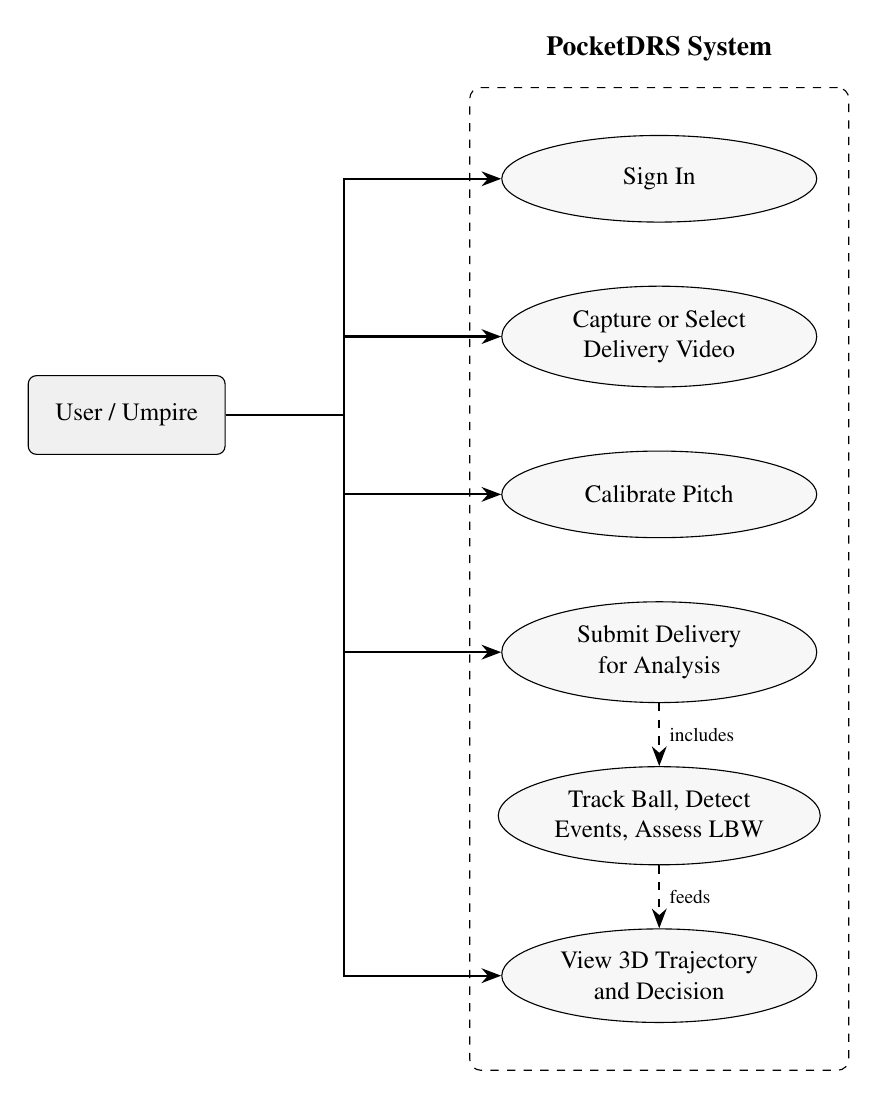
\begin{tikzpicture}[
    node distance=1.0cm and 2.5cm,
    entity/.style={draw, rounded corners=3pt, minimum width=2.5cm, minimum height=1cm, align=center, font=\small, fill=gray!12},
    usecase/.style={draw, ellipse, minimum width=4cm, minimum height=1.1cm, align=center, font=\small, fill=gray!6},
    sys/.style={draw, dashed, rounded corners=4pt, inner xsep=0.4cm, inner ysep=0.6cm},
    rel/.style={-{Stealth[length=2.5mm]}, line width=0.8pt},
    note/.style={font=\scriptsize, align=center}
]

\node[entity] (user) {User / Umpire};

\node[usecase, right=3.5cm of user, yshift=3.0cm] (u1) {Sign In};
\node[usecase, below=0.8cm of u1] (u2) {Capture or Select\\Delivery Video};
\node[usecase, below=0.8cm of u2] (u3) {Calibrate Pitch};
\node[usecase, below=0.8cm of u3] (u4) {Submit Delivery\\for Analysis};
\node[usecase, below=0.8cm of u4] (u5) {Track Ball, Detect\\Events, Assess LBW};
\node[usecase, below=0.8cm of u5] (u6) {View 3D Trajectory\\and Decision};

\node[sys, fit=(u1)(u6), label={[font=\bfseries, yshift=2mm]above:PocketDRS System}] (sysbox) {};

\draw[rel] (user.east) -- ++(1.5,0) |- (u1.west);
\draw[rel] (user.east) -- ++(1.5,0) |- (u2.west);
\draw[rel] (user.east) -- ++(1.5,0) |- (u3.west);
\draw[rel] (user.east) -- ++(1.5,0) |- (u4.west);
\draw[rel] (user.east) -- ++(1.5,0) |- (u6.west);

\draw[dashed, rel] (u4.south) -- node[note, right] {includes} (u5.north);
\draw[dashed, rel] (u5.south) -- node[note, right] {feeds} (u6.north);
\end{tikzpicture}
}
\caption{Main use cases of PocketDRS.}
\label{fig:usecase}
\end{figure}

\subsection{Feasibility Study}

\subsubsection{Technical Feasibility}

The current prototype uses tools that are already stable and widely used. Flutter handles the mobile app. FastAPI handles the server API. OpenCV handles video analysis. Three.js is used for the 3D result view inside a WebView. This stack is realistic for a student project and works on consumer hardware.

\subsubsection{Operational Feasibility}

The workflow is simple enough for normal use. A phone on a tripod records the ball. The user marks pitch points once, trims the clip, and waits for the result. The steps are short and easy to repeat during testing.

\subsubsection{Economic Feasibility}

The project does not need special sensors or paid software. It uses open source libraries and devices that are already available. That keeps the cost very low.

\begin{table}[htbp]
\centering
\caption{Main tools used in PocketDRS.}
\label{tab:stack}
\begin{tabularx}{\textwidth}{@{}lX@{}}
\toprule
\textbf{Part} & \textbf{Tool} \\
\midrule
Mobile app & Flutter and Dart \\
Server API & FastAPI and Python \\
Vision pipeline & OpenCV, NumPy, SciPy \\
Authentication & Firebase Authentication \\
Data storage & Cloud Firestore \\
3D result view & Three.js inside WebView \\
Testing & pytest and Flutter analyzer \\
\bottomrule
\end{tabularx}
\end{table}

\subsection{High Level Design of System}

The design can be understood through the following views: overall system architecture, context-level data flow, level-1 processing flow, application activity flow, software components, and deployment structure. Together these diagrams show how PocketDRS moves from user input to final LBW decision output.

\begin{figure}[htbp]
\centering
\resizebox{0.6\textwidth}{!}{%
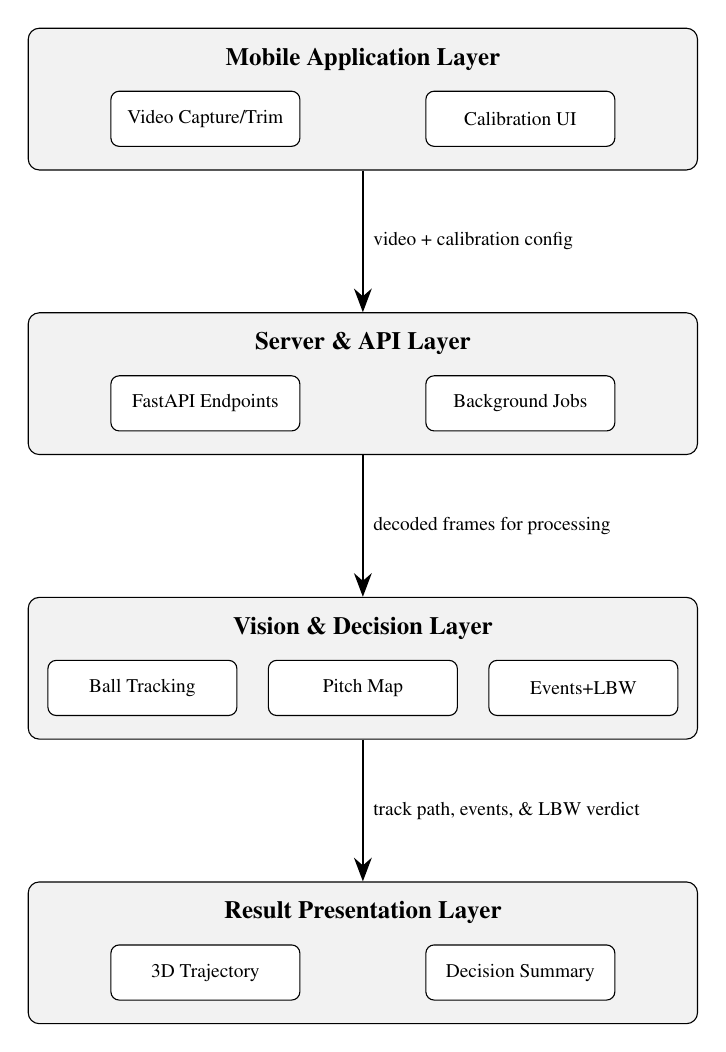
\begin{tikzpicture}[
    node distance=1.5cm,
    layer/.style={draw, rounded corners=4pt, minimum width=8.5cm, minimum height=1.8cm, align=center, font=\small, fill=gray!10},
    smallbox/.style={draw, rounded corners=3pt, minimum width=2.4cm, minimum height=0.7cm, align=center, font=\scriptsize, fill=white},
    flow/.style={-{Stealth[length=3mm]}, line width=0.9pt}
]

\node[layer] (mobile) {};
\node[font=\small\bfseries] at (mobile.north) [yshift=-4mm] {Mobile Application Layer};
\node[smallbox] (m1) at ([xshift=-2.0cm,yshift=-2.5mm]mobile.center) {Video Capture/Trim};
\node[smallbox] (m2) at ([xshift=2.0cm,yshift=-2.5mm]mobile.center) {Calibration UI};

\node[layer, below=1.8cm of mobile] (api) {};
\node[font=\small\bfseries] at (api.north) [yshift=-4mm] {Server \& API Layer};
\node[smallbox] (a1) at ([xshift=-2.0cm,yshift=-2.5mm]api.center) {FastAPI Endpoints};
\node[smallbox] (a2) at ([xshift=2.0cm,yshift=-2.5mm]api.center) {Background Jobs};

\node[layer, below=1.8cm of api] (pipeline) {};
\node[font=\small\bfseries] at (pipeline.north) [yshift=-4mm] {Vision \& Decision Layer};
\node[smallbox] (p1) at ([xshift=-2.8cm,yshift=-2.5mm]pipeline.center) {Ball Tracking};
\node[smallbox] (p2) at ([xshift=0,yshift=-2.5mm]pipeline.center) {Pitch Map};
\node[smallbox] (p3) at ([xshift=2.8cm,yshift=-2.5mm]pipeline.center) {Events+LBW};

\node[layer, below=1.8cm of pipeline] (result) {};
\node[font=\small\bfseries] at (result.north) [yshift=-4mm] {Result Presentation Layer};
\node[smallbox] (r1) at ([xshift=-2.0cm,yshift=-2.5mm]result.center) {3D Trajectory};
\node[smallbox] (r2) at ([xshift=2.0cm,yshift=-2.5mm]result.center) {Decision Summary};

\draw[flow] (mobile.south) -- node[right, font=\scriptsize, align=center] {video + calibration config} (api.north);
\draw[flow] (api.south) -- node[right, font=\scriptsize, align=center] {decoded frames for processing} (pipeline.north);
\draw[flow] (pipeline.south) -- node[right, font=\scriptsize, align=center] {track path, events, \& LBW verdict} (result.north);
\end{tikzpicture}
}
\caption{Overall architecture of PocketDRS.}
\label{fig:highlevel}
\end{figure}

\subsubsection{Context Level DFD}

\begin{figure}[htbp]
\centering
\resizebox{0.96\textwidth}{!}{%
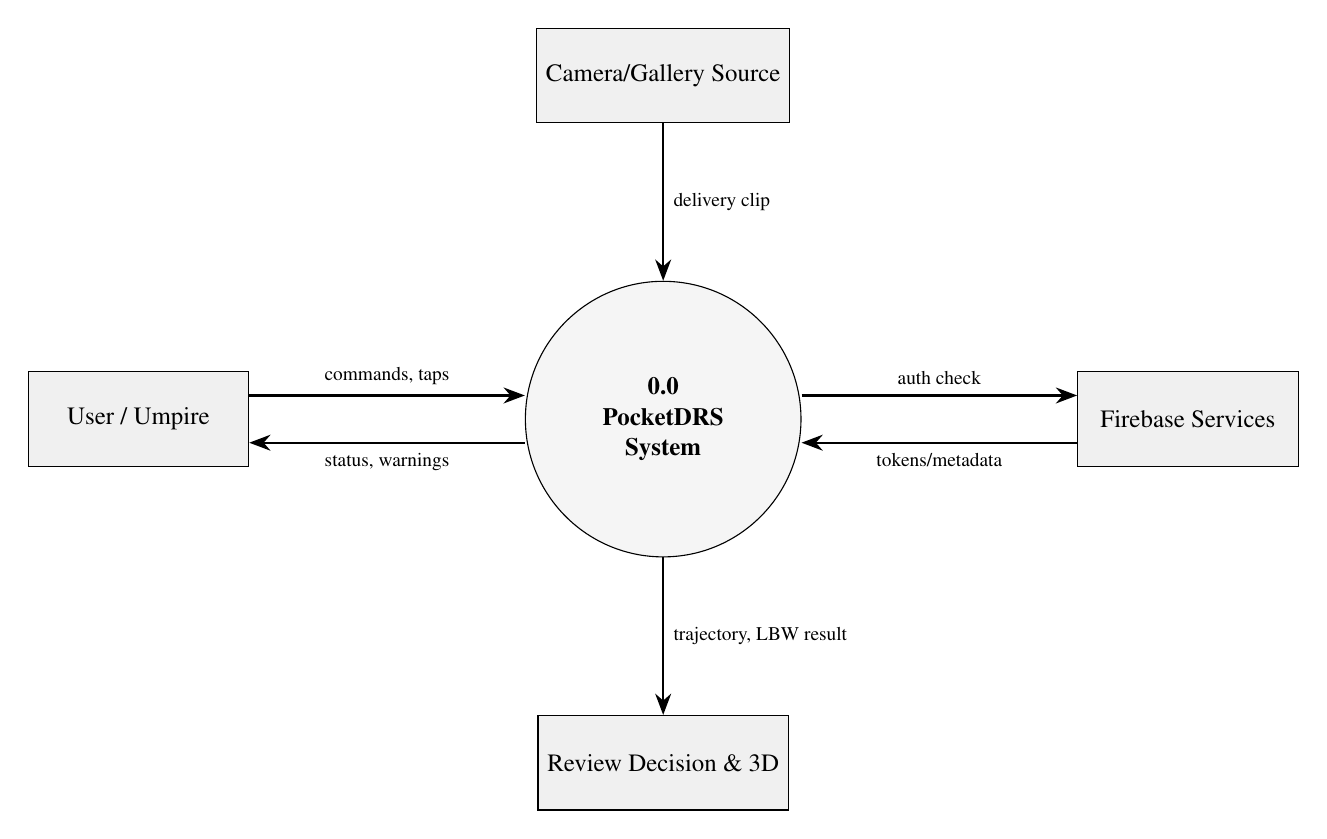
\begin{tikzpicture}[
    node distance=2.5cm and 3.5cm,
    ext/.style={draw, minimum width=2.8cm, minimum height=1.2cm, align=center, font=\small, fill=gray!12},
    proc/.style={draw, circle, minimum size=3.5cm, align=center, font=\small\bfseries, fill=gray!8},
    data/.style={-{Stealth[length=2.7mm]}, line width=0.8pt},
    lbl/.style={font=\scriptsize, align=center}
]

\node[proc] (system) {0.0\\PocketDRS\\System};
\node[ext, left=3.5cm of system] (user) {User / Umpire};
\node[ext, above=2cm of system] (media) {Camera/Gallery Source};
\node[ext, right=3.5cm of system] (firebase) {Firebase Services};
\node[ext, below=2cm of system] (result) {Review Decision \& 3D};

\draw[data, transform canvas={yshift=3mm}] (user.east) -- node[lbl, above] {commands, taps} (system.west);
\draw[data, transform canvas={yshift=-3mm}] (system.west) -- node[lbl, below] {status, warnings} (user.east);
\draw[data] (media.south) -- node[lbl, right] {delivery clip} (system.north);
\draw[data, transform canvas={yshift=3mm}] (system.east) -- node[lbl, above] {auth check} (firebase.west);
\draw[data, transform canvas={yshift=-3mm}] (firebase.west) -- node[lbl, below] {tokens/metadata} (system.east);
\draw[data] (system.south) -- node[lbl, right] {trajectory, LBW result} (result.north);
\end{tikzpicture}
}
\caption{Context-level DFD of PocketDRS.}
\label{fig:dfd-context}
\end{figure}

\subsubsection{Level 1 DFD}

\begin{figure}[htbp]
\centering
\resizebox{0.96\textwidth}{!}{%
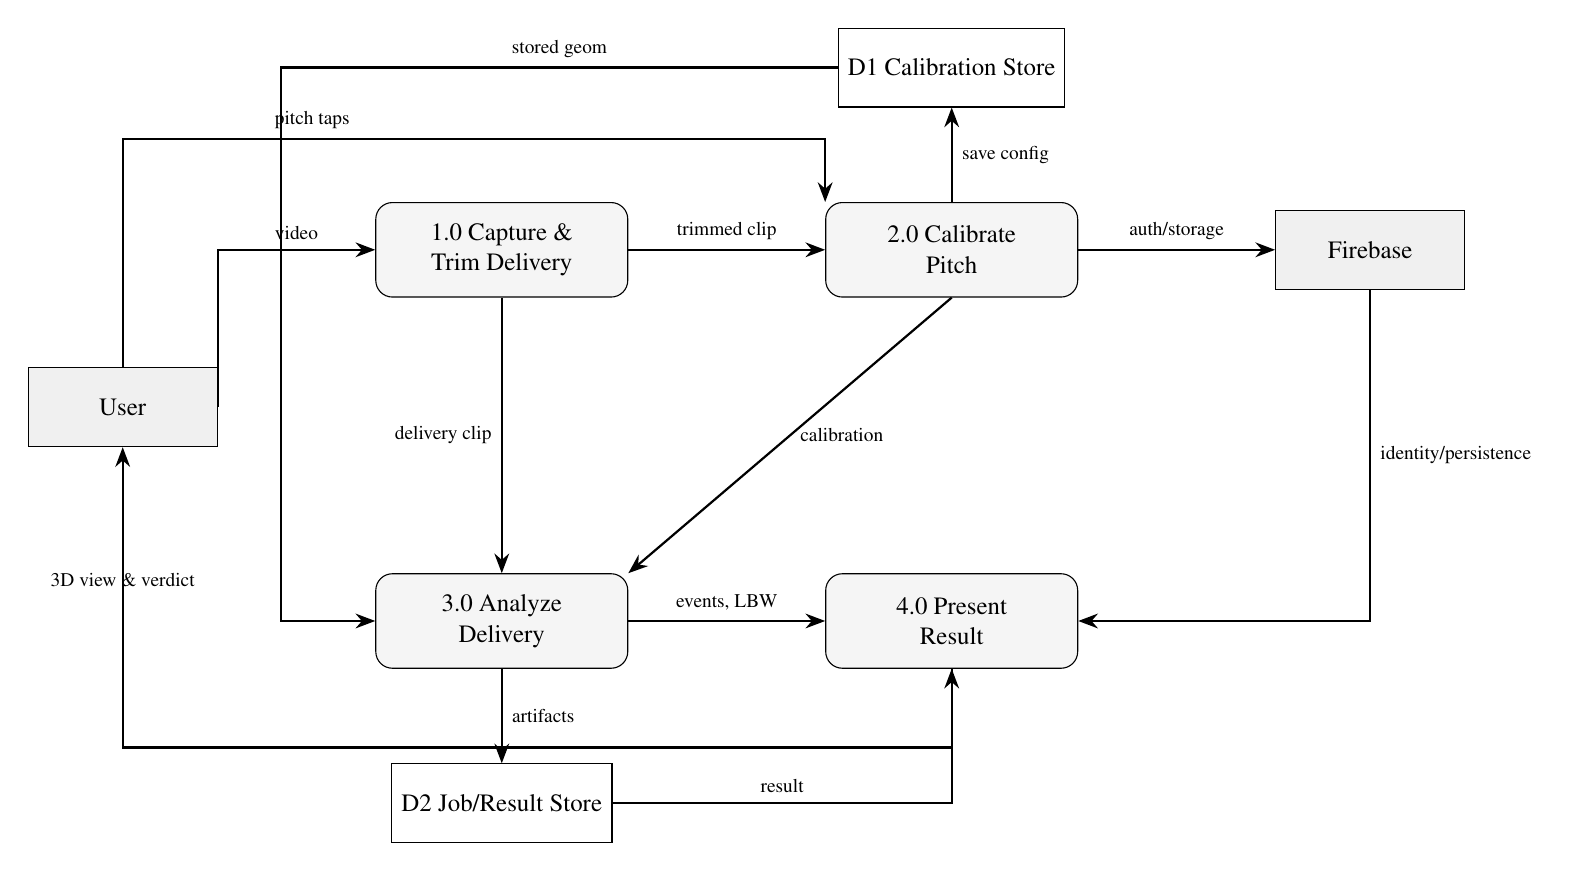
\begin{tikzpicture}[
    node distance=1.5cm and 2cm,
    ext/.style={draw, minimum width=2.4cm, minimum height=1cm, align=center, font=\small, fill=gray!12},
    proc/.style={draw, rounded corners=6pt, minimum width=3.2cm, minimum height=1.2cm, align=center, font=\small, fill=gray!8},
    store/.style={draw, minimum width=2.8cm, minimum height=1cm, align=center, font=\small, fill=white},
    flow/.style={-{Stealth[length=2.5mm]}, line width=0.8pt},
    lbl/.style={font=\scriptsize, align=center}
]

\node[ext] (user) {User};
\node[proc, right=2.0cm of user, yshift=2.0cm] (p1) {1.0 Capture \&\\Trim Delivery};
\node[proc, right=2.5cm of p1] (p2) {2.0 Calibrate\\Pitch};
\node[ext, right=2.5cm of p2] (firebase) {Firebase};

\node[proc, below=3.5cm of p1] (p3) {3.0 Analyze\\Delivery};
\node[proc, below=3.5cm of p2] (p4) {4.0 Present\\Result};

\node[store, above=1.2cm of p2] (d1) {D1 Calibration Store};
\node[store, below=1.2cm of p3] (d2) {D2 Job/Result Store};

\draw[flow] (user.east) |- node[lbl, above, pos=0.75] {video} (p1.west);
\draw[flow] (user.north) |- node[lbl, above, near end] {pitch taps} ([yshift=8mm]p1.north) -| (p2.north west);

\draw[flow] (p1.east) -- node[lbl, above] {trimmed clip} (p2.west);
\draw[flow] (p2.north) -- node[lbl, right] {save config} (d1.south);
\draw[flow] (p2.south) -- node[lbl, right] {calibration} (p3.north east);
\draw[flow] (p1.south) -- node[lbl, left] {delivery clip} (p3.north);

\draw[flow] (d1.west) -| node[lbl, near start, above] {stored geom} ([xshift=-1.2cm]p1.west) |- (p3.west);

\draw[flow] (p3.east) -- node[lbl, above] {events, LBW} (p4.west);
\draw[flow] (p3.south) -- node[lbl, right] {artifacts} (d2.north);
\draw[flow] (d2.east) -| node[lbl, near start, above] {result} (p4.south);

\draw[flow] (p2.east) -- node[lbl, above] {auth/storage} (firebase.west);
\draw[flow] (firebase.south) |- node[lbl, right, near start] {identity/persistence} (p4.east);

\draw[flow] (p4.south) |- ++(0,-1cm) -| node[lbl, above, near end] {3D view \& verdict} (user.south);
\end{tikzpicture}
}
\caption{Level-1 DFD of the PocketDRS processing workflow.}
\label{fig:dfd-level1}
\end{figure}

\subsubsection{Working Flow}

The working flow is kept short so that the user can follow it easily:

\begin{figure}[htbp]
\centering
\resizebox{0.96\textwidth}{!}{%
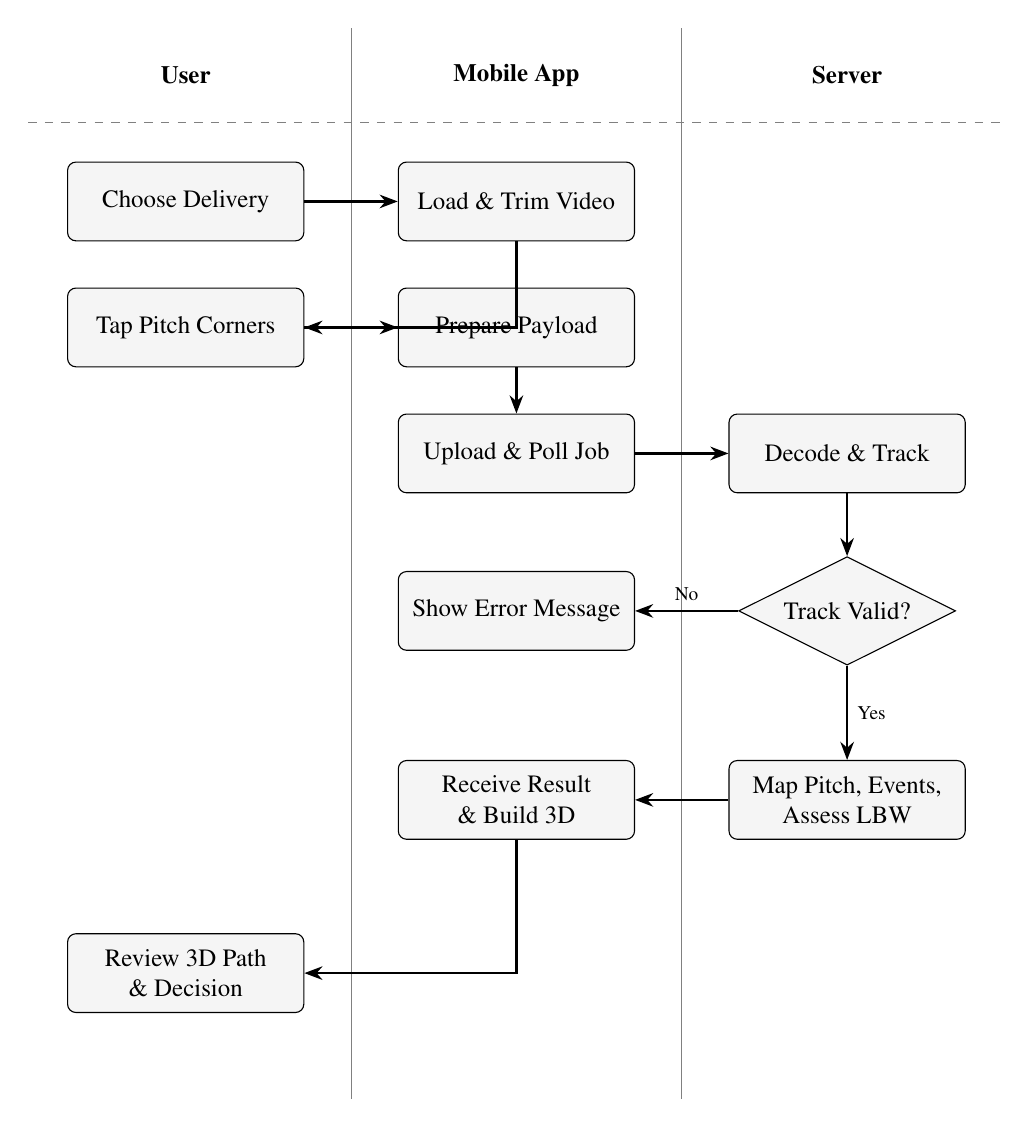
\begin{tikzpicture}[
    node distance=1.0cm and 1.5cm,
    head/.style={font=\small\bfseries, align=center},
    flowstep/.style={draw, rounded corners=3pt, minimum width=3.0cm, minimum height=1.0cm, align=center, font=\small, fill=gray!8},
    decision/.style={draw, diamond, aspect=2.0, minimum width=2.6cm, align=center, font=\small, fill=gray!8},
    arrow/.style={-{Stealth[length=2.3mm]}, line width=0.8pt}
]

\def\w{4.2}
\node[head] (h1) at (-\w, 0) {User};
\node[head] (h2) at (0, 0) {Mobile App};
\node[head] (h3) at (\w, 0) {Server};

\draw[dashed, gray] (-\w-2.0, -0.6) -- (\w+2.0, -0.6);
\draw[gray] (-0.5*\w, 0.6) -- (-0.5*\w, -13.0);
\draw[gray] (0.5*\w, 0.6) -- (0.5*\w, -13.0);

\node[flowstep] (u1) at (-\w, -1.6) {Choose Delivery};
\node[flowstep] (a1) at (0, -1.6) {Load \& Trim Video};
\node[flowstep] (u2) at (-\w, -3.2) {Tap Pitch Corners};
\node[flowstep] (a2) at (0, -3.2) {Prepare Payload};
\node[flowstep] (a3) at (0, -4.8) {Upload \& Poll Job};
\node[flowstep] (s1) at (\w, -4.8) {Decode \& Track};
\node[decision] (s2) at (\w, -6.8) {Track Valid?};
\node[flowstep] (a5) at (0, -6.8) {Show Error Message};
\node[flowstep] (s3) at (\w, -9.2) {Map Pitch, Events,\\Assess LBW};
\node[flowstep] (a4) at (0, -9.2) {Receive Result\\\& Build 3D};
\node[flowstep] (u3) at (-\w, -11.4) {Review 3D Path\\\& Decision};

\draw[arrow] (u1.east) -- (a1.west);
\draw[arrow] (a1.south) |- (u2.east);
\draw[arrow] (u2.east) -- (a2.west);
\draw[arrow] (a2.south) -- (a3.north);
\draw[arrow] (a3.east) -- (s1.west);
\draw[arrow] (s1.south) -- (s2.north);
\draw[arrow] (s2.west) -- node[above, font=\scriptsize] {No} (a5.east);
\draw[arrow] (s2.south) -- node[right, font=\scriptsize, align=center] {Yes} (s3.north);
\draw[arrow] (s3.west) -- (a4.east);
\draw[arrow] (a4.south) |- (u3.east);
\end{tikzpicture}
}
\caption{Main processing flow used by the system.}
\label{fig:activity}
\end{figure}

\subsubsection{System Components}

\begin{figure}[htbp]
\centering
\resizebox{0.96\textwidth}{!}{%
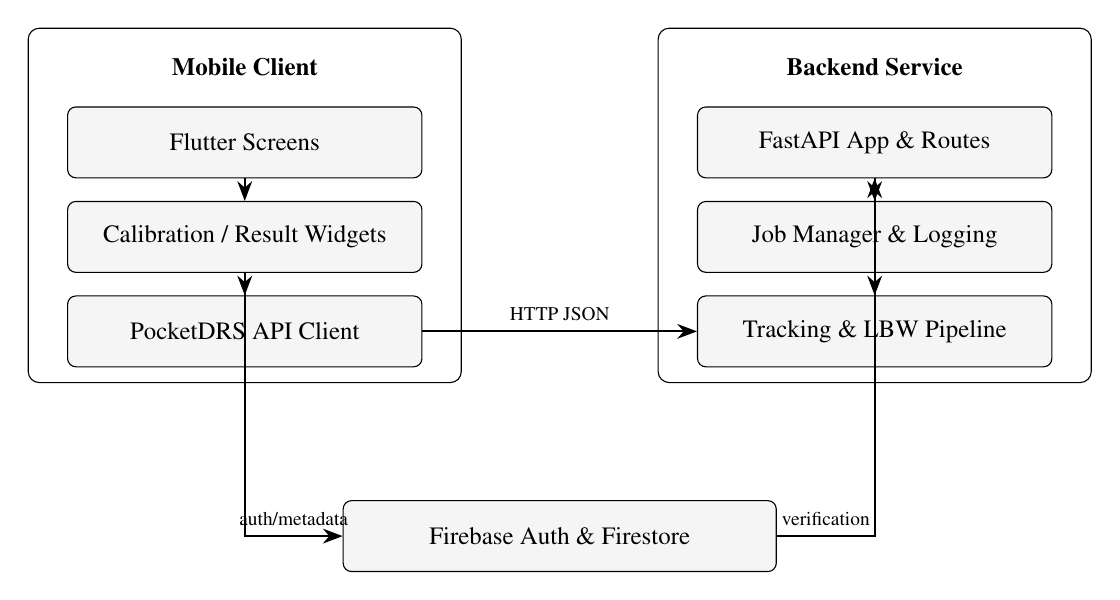
\begin{tikzpicture}[
    node distance=1.0cm and 2.5cm,
    pkg/.style={draw, rounded corners=4pt, minimum width=5.5cm, minimum height=4.5cm},
    comp/.style={draw, rounded corners=3pt, minimum width=4.5cm, minimum height=0.9cm, align=center, font=\small, fill=gray!8},
    arrow/.style={-{Stealth[length=2.5mm]}, line width=0.8pt},
    lbl/.style={font=\scriptsize, align=center}
]

\node[pkg] (mobile) at (-4, 0) {};
\node[font=\small\bfseries] at (mobile.north) [yshift=-5mm] {Mobile Client};
\node[comp] (c1) at (-4, 0.8) {Flutter Screens};
\node[comp] (c2) at (-4, -0.4) {Calibration / Result Widgets};
\node[comp] (c3) at (-4, -1.6) {PocketDRS API Client};

\node[pkg] (backend) at (4, 0) {};
\node[font=\small\bfseries] at (backend.north) [yshift=-5mm] {Backend Service};
\node[comp] (b1) at (4, 0.8) {FastAPI App \& Routes};
\node[comp] (b2) at (4, -0.4) {Job Manager \& Logging};
\node[comp] (b3) at (4, -1.6) {Tracking \& LBW Pipeline};

\node[comp, minimum width=5.5cm] (firebase) at (0, -4.2) {Firebase Auth \& Firestore};

\draw[arrow] (c1.south) -- (c2.north);
\draw[arrow] (c2.south) -- (c3.north);

\draw[arrow] (b1.south) -- (b2.north);
\draw[arrow] (b2.south) -- (b3.north);

\draw[arrow] (c3.east) -- node[lbl, above] {HTTP JSON} (b3.west |- c3.east);

\draw[arrow] (c2.south) |- node[lbl, above, near end] {auth/metadata} (firebase.west);
\draw[arrow] (firebase.east) -| node[lbl, above, near start] {verification} (b1.south);
\end{tikzpicture}
}
\caption{Main software components.}
\label{fig:component}
\end{figure}

\subsubsection{Deployment View}

\begin{figure}[htbp]
\centering
\resizebox{0.96\textwidth}{!}{%
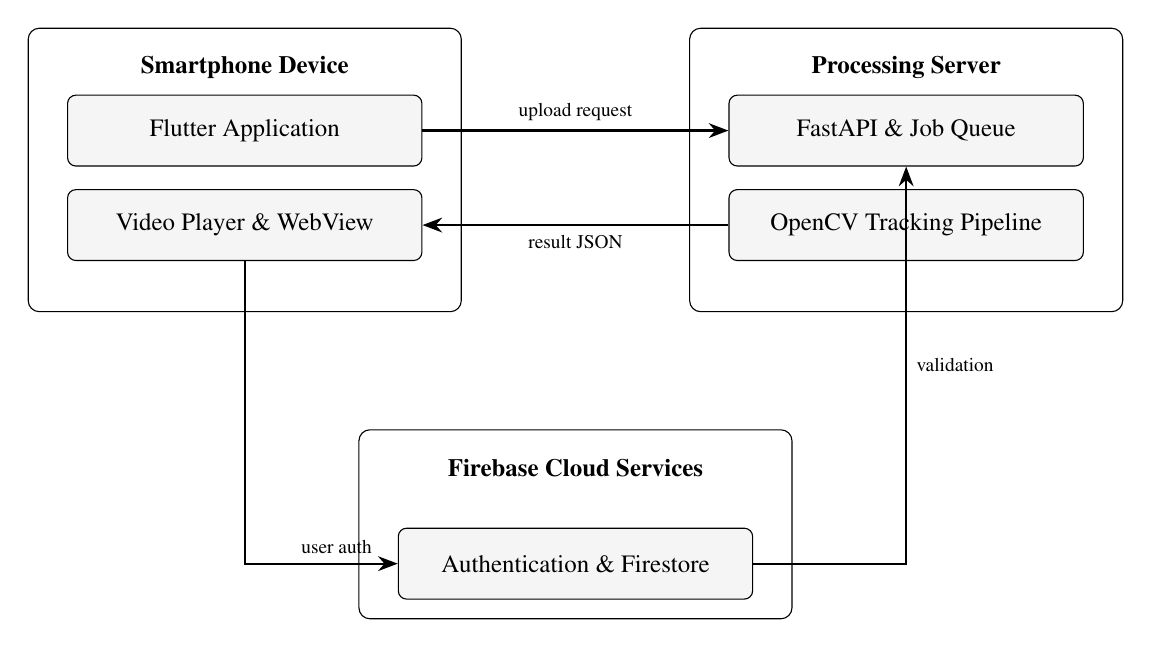
\begin{tikzpicture}[
    node distance=1.5cm and 3cm,
    nodebox/.style={draw, rounded corners=4pt, minimum width=5.5cm, minimum height=3.6cm, align=center, font=\small},
    inner/.style={draw, rounded corners=3pt, minimum width=4.5cm, minimum height=0.9cm, align=center, font=\small, fill=gray!8},
    arrow/.style={-{Stealth[length=2.5mm]}, line width=0.8pt},
    lbl/.style={font=\scriptsize, align=center}
]

\node[nodebox] (phone) at (-4.2, 0) {};
\node[font=\small\bfseries] at (phone.north) [yshift=-5mm] {Smartphone Device};
\node[inner] (m1) at (-4.2, 0.5) {Flutter Application};
\node[inner] (m2) at (-4.2, -0.7) {Video Player \& WebView};

\node[nodebox] (server) at (4.2, 0) {};
\node[font=\small\bfseries] at (server.north) [yshift=-5mm] {Processing Server};
\node[inner] (s1) at (4.2, 0.5) {FastAPI \& Job Queue};
\node[inner] (s2) at (4.2, -0.7) {OpenCV Tracking Pipeline};

\node[nodebox, minimum height=2.4cm] (cloud) at (0, -4.5) {};
\node[font=\small\bfseries] at (cloud.north) [yshift=-5mm] {Firebase Cloud Services};
\node[inner] (f1) at (0, -5.0) {Authentication \& Firestore};

\draw[arrow] (m1.east) -- node[lbl, above] {upload request} (s1.west);
\draw[arrow] (s2.west) -- node[lbl, below] {result JSON} (m2.east);

\draw[arrow] (m2.south) |- node[lbl, above, pos=0.8] {user auth} (f1.west);
\draw[arrow] (f1.east) -| node[lbl, right, near end] {validation} (s1.south);

\end{tikzpicture}
}
\caption{Deployment view of the working system.}
\label{fig:deployment}
\end{figure}

\subsubsection{Current Implementation Status}

The project is not only planned on paper. A working prototype already exists and has gone through a full cycle of implementation and improvement. Below is the current state of each part of the system.

\textbf{Mobile Application.} The Flutter app supports sign in with Firebase, video selection and recording, an interactive pitch calibration step where the user taps four pitch corners and two stump bases, video trimming, submission to the server, live progress polling, and a full result screen with a 3D trajectory view. The calibration screen validates user inputs and checks for geometric consistency before allowing the user to proceed.

\textbf{Server and API.} The FastAPI server accepts video uploads and processes them as background jobs. Each job goes through frame decoding, ball tracking, calibration mapping, bounce and impact detection, and LBW assessment. The job API returns structured results including track points, pitch plane coordinates, event indices, and an LBW decision with reasons.

\textbf{Ball Tracking Pipeline.} Tracking uses a combined motion and colour detection approach. A MOG2 background subtractor detects moving objects while an HSV colour detector finds the ball by its known colour. The two detectors are fused so that matches between them receive higher confidence. A recent improvement adds a region-of-interest (ROI) mask built from the calibration corners, which restricts detection to the pitch area and its surroundings. This eliminates false positives from fielders, boundary boards, and camera shake in the background.

\textbf{Pitch Calibration and Homography.} The user marks four pitch corners and two stump bases on a reference frame. The server uses these to compute a homography matrix that maps pixel positions to real pitch coordinates. Stump base points refine the homography. A reprojection quality score warns the user when calibration may be inaccurate.

\textbf{Event Detection and LBW.} Bounce and impact events are detected using both pixel-space and pitch-plane heuristics. The system looks for velocity changes and lateral direction shifts to identify the bounce point, and finds the first point near the striker crease as impact. The LBW module fits a curve through the post-bounce trajectory and evaluates where the ball would cross the stump line. It checks pitching in line, impact in line, and whether the ball would hit the stumps, and reports a decision with a confidence metric.

\textbf{3D Visualization.} The result view uses Three.js loaded in a WebView. It renders a realistic cricket pitch with stumps, crease lines, and the ball trajectory as coloured tubes (blue before bounce, green after bounce, amber for the predicted path). Bounce and impact points are shown as highlighted markers. The user can rotate the view using touch controls.

\section{Gantt Chart}

\begin{table}[htbp]
\centering
\caption{Project schedule.}
\label{tab:gantt}
\begin{tabularx}{\textwidth}{@{}Xccccc@{}}
\toprule
\textbf{Task} & \textbf{Dec} & \textbf{Jan} & \textbf{Feb} & \textbf{Mar} & \textbf{Apr} \\
\midrule
Problem study and review & X & X &  &  &  \\
System design &  & X & X &  &  \\
App and server development &  & X & X & X &  \\
Tracking and decision logic &  &  & X & X &  \\
Testing and refinement &  &  &  & X & X \\
Final improvement and report work &  &  &  & X & X \\
\bottomrule
\end{tabularx}
\end{table}

\section{Expected Outcome}

The expected outcome of PocketDRS is a working low-cost review tool for cricket that can:

\begin{enumerate}
    \item Accept a single delivery clip from a phone.
    \item Map the video to the cricket pitch using user selected points.
    \item Track the ball through the important part of the delivery.
    \item Mark bounce and impact in a useful way.
    \item Give a simple LBW decision with a clear visual result.
    \item Help clubs and student level cricket use a DRS-like tool without expensive equipment.
\end{enumerate}

If accuracy improves further with more testing data, the same system can later grow into a stronger tool for coaching, match review, and training support.

\section{References}

\begin{thebibliography}{99}

\bibitem{hawkeye2024}
Hawk-Eye Innovations, ``Hawk-Eye: The Technology Behind Sports Officiating,'' 2024. [Online]. Available: \url{https://www.hawkeyeinnovations.com/}

\bibitem{ponglertnapakorn2021}
P. Ponglertnapakorn, T. Shirai, and T. Yamasaki, ``Where Is the Ball: 3D Ball Trajectory Estimation From 2D Monocular Tracking,'' in \textit{Proceedings of the IEEE/CVF Conference on Computer Vision and Pattern Recognition}, 2021.

\bibitem{zhang2000}
Z. Zhang, ``A Flexible New Technique for Camera Calibration,'' \textit{IEEE Transactions on Pattern Analysis and Machine Intelligence}, vol. 22, no. 11, pp. 1330--1334, 2000.

\bibitem{opencv2024}
OpenCV Documentation, ``Camera Calibration and 3D Reconstruction,'' 2024. [Online]. Available: \url{https://docs.opencv.org/}

\bibitem{icc_rules}
International Cricket Council, ``Playing Conditions: Law 36 Leg Before Wicket,'' 2024.

\bibitem{flutter2024}
Google, ``Flutter: Build apps for any screen,'' 2024. [Online]. Available: \url{https://flutter.dev/}

\bibitem{fastapi2024}
S. Ram\'{i}rez, ``FastAPI: Modern, fast web framework for building APIs with Python,'' 2024. [Online]. Available: \url{https://fastapi.tiangolo.com/}

\bibitem{threejs2024}
Three.js Contributors, ``Three.js: JavaScript 3D Library,'' 2024. [Online]. Available: \url{https://threejs.org/}

\end{thebibliography}

\end{document}
